\documentclass[10pt, aspectratio=169]{beamer}

\usepackage[utf8]{inputenc}
\usepackage[T1]{fontenc}
\usepackage[french]{babel}
\usepackage{graphicx}
\usepackage{booktabs}
\usepackage{xcolor}
\usepackage{colortbl}

\usetheme{Madrid}
\usecolortheme{default}

% --- Couleurs personnalisees ---
\definecolor{uqblue}{RGB}{21,101,192}
\setbeamercolor{structure}{fg=uqblue}
\setbeamercolor{frametitle}{bg=uqblue, fg=white}
\setbeamercolor{title}{fg=uqblue}
\setbeamertemplate{itemize items}[circle]

\title[Prédiction Séries Temporelles]{Hackathon : Prédiction de Séries Temporelles Financières}
\subtitle{Pipeline Deep Learning Multi-Actifs}
\author{Louis Cluzel}
\institute[UCA]{M1 Intelligence Artificielle -- Université Clermont Auvergne}
\date{Avril 2026}

\begin{document}

% ---------------------------------------------------------
\begin{frame}[plain]
    \titlepage
\end{frame}

% ---------------------------------------------------------
\begin{frame}{Le Défi}
    \textbf{Objectif :} Prédire à l'horizon de \alert{15 pas de temps} l'évolution de deux indicateurs techniques très utilisés en trading quantitatif.
    
    \vspace{0.5cm}
    \begin{columns}
        \column{0.6\textwidth}
        \begin{block}{Indicateurs Cibles}
            \begin{itemize}
                \item \textbf{MACD (12, 26, 9)} : Mesure l'inertie et la tendance.
                \item \textbf{Stochastique \%K (14, 3, 5)} : Oscillateur de Momentum.
            \end{itemize}
        \end{block}
        
        \vspace{0.3cm}
        \textbf{Évaluation (Score Hackathon)} $\geq 0.55$ \\
        Formule équilibrant direction temporelle ($T$) et corrélation de Pearson ($\rho$) sur les deux courbes.

        \column{0.4\textwidth}
        \centering
        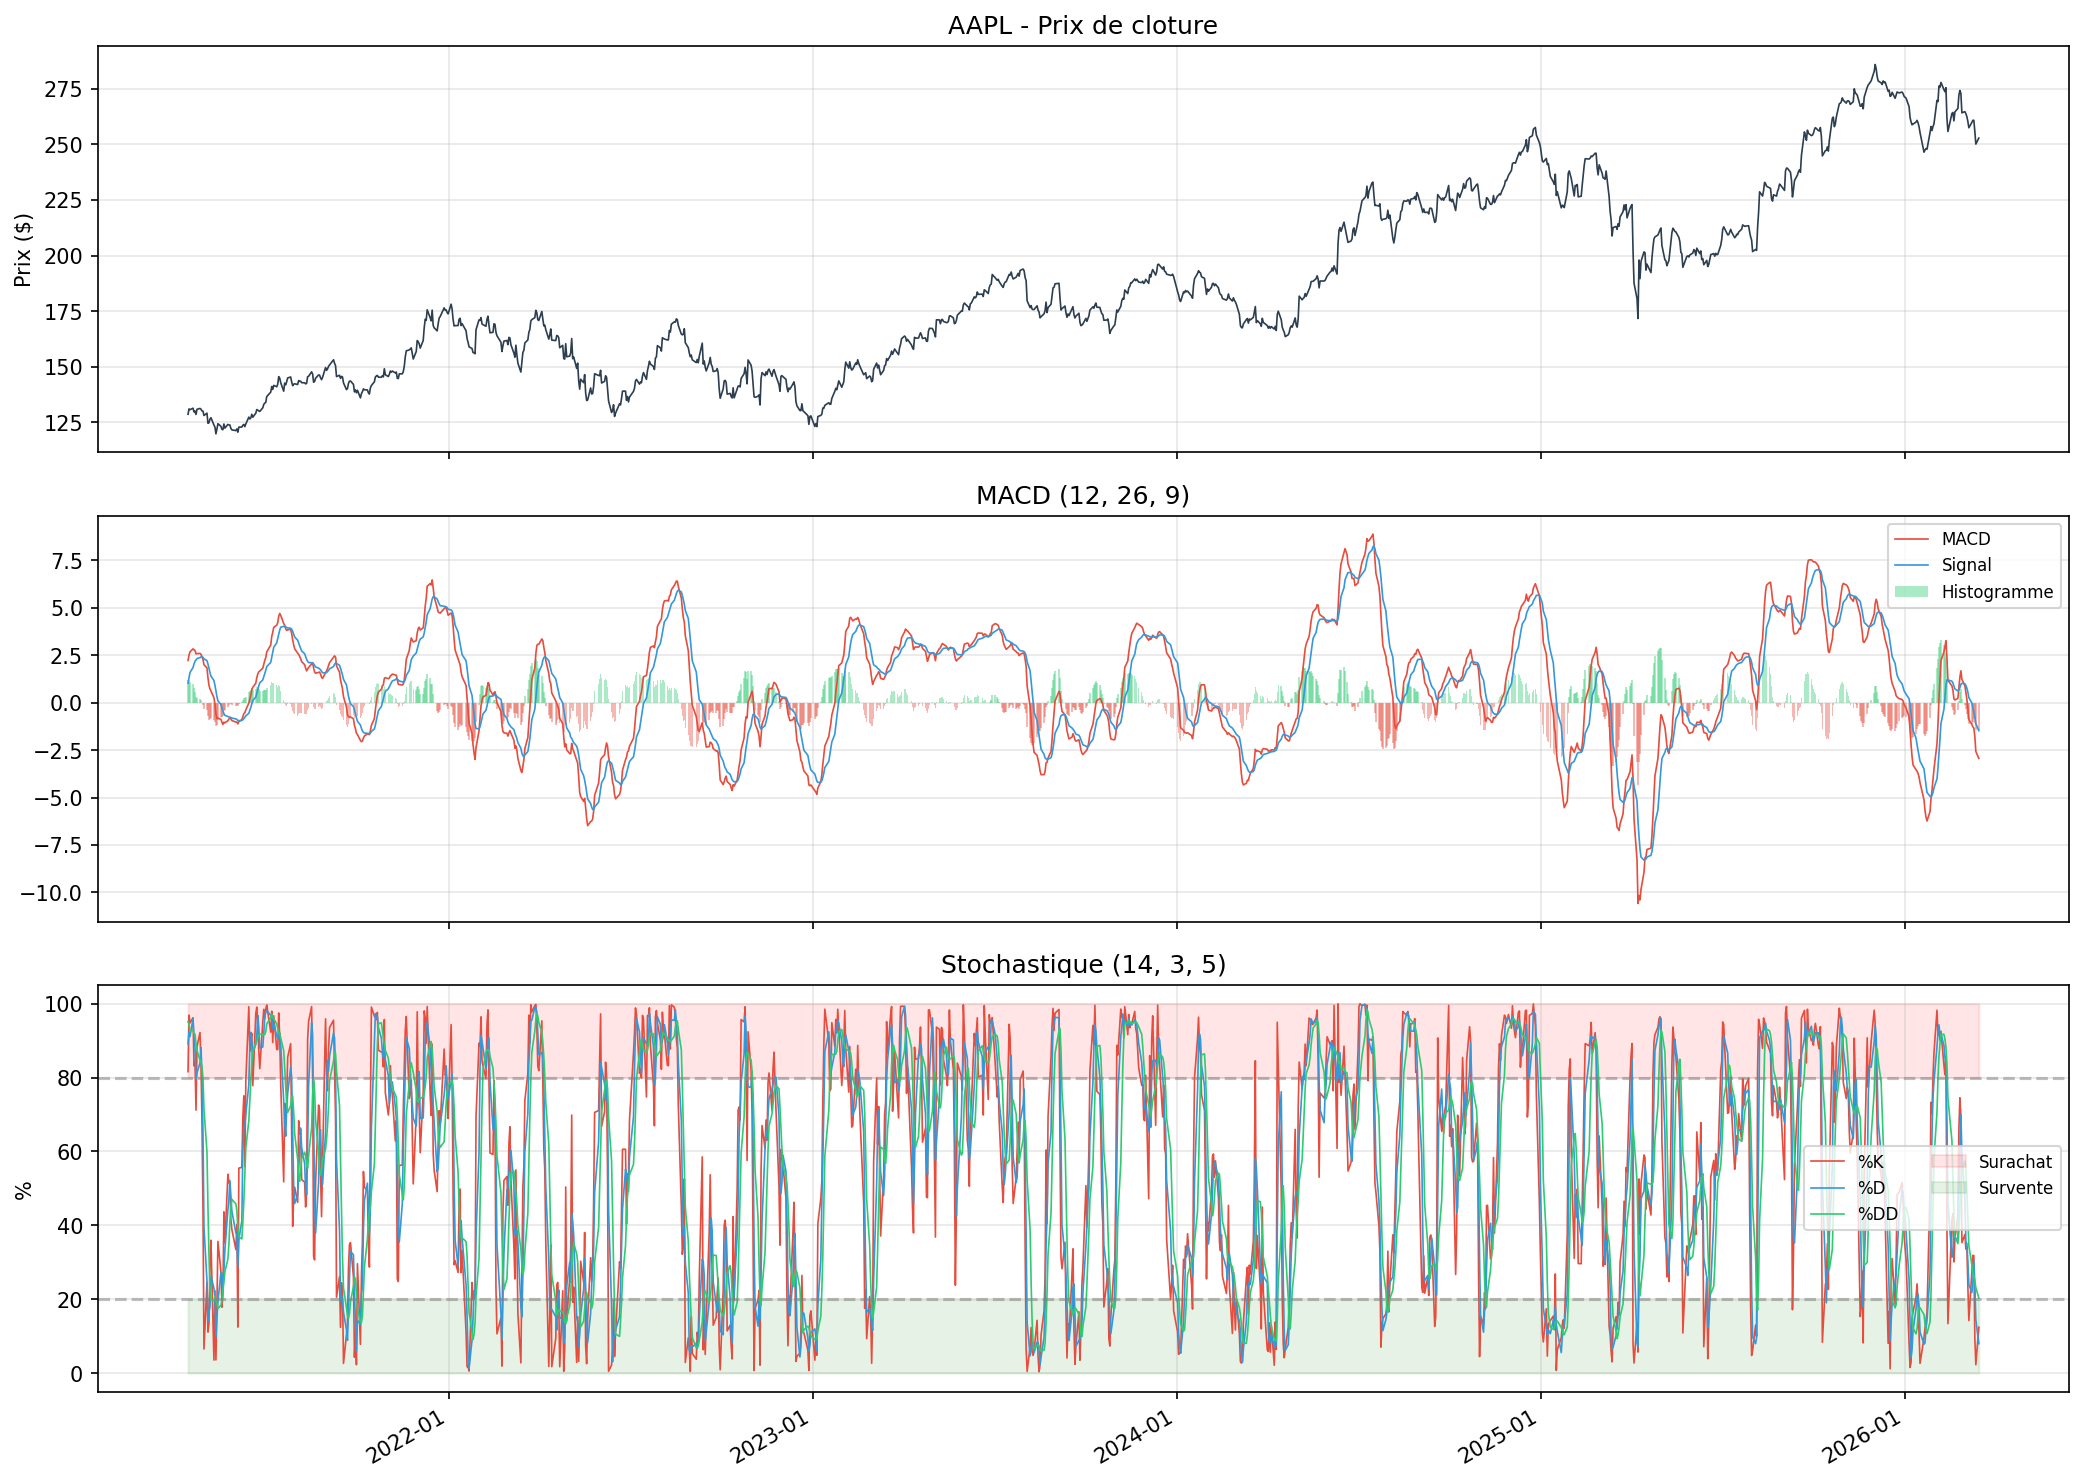
\includegraphics[width=0.9\textwidth]{../figures/AAPL_indicators_overview.png}
    \end{columns}
\end{frame}

% ---------------------------------------------------------
\begin{frame}{Pipeline \& Feature Engineering}
    \textbf{Question :} Comment un pas de temps historique pénètre-t-il le réseau ?

    \vspace{0.5cm}
    \begin{columns}
        \column{0.5\textwidth}
        Chaque observation boursière est décomposée en un vecteur de \textbf{5 composantes normées} :
        \begin{itemize}
            \item Valeur courante MinMax
            \item Rendement relatif au close
            \item Moyenne mobile EMA 10
            \item Moyenne mobile EMA 20
            \item Volatilité locale (Écart-type 10)
        \end{itemize}

        \column{0.5\textwidth}
        \begin{block}{Le Rôle du Lookback ($L=120$)}
            Plutôt que des données brutes, une fenêtre glissante de 120 pas chronologiques encapsule ces vecteurs pour alimenter massivement le tenseur du réseau !
        \end{block}
    \end{columns}
\end{frame}

% ---------------------------------------------------------
\begin{frame}{Approche Multi-Actifs}
    Au lieu de su-entraîner le modèle sur l'unique fichier test fourni, l'architecture assume une versatilité parfaite via \textbf{3 actifs extrêmes} :

    \vspace{0.5cm}
    \begin{columns}
        \column{0.3\textwidth}
        \centering
        \textbf{Apple (AAPL)} \\
        \vspace{0.2cm}
        Intraday (5 min)\\
        94 334 barres\\
        {\small \color{gray}(Hyper-régularité)}

        \column{0.3\textwidth}
        \centering
        \textbf{Microsoft (MSFT)} \\
        \vspace{0.2cm}
        Journalier\\
        $\sim$ 1 200 jours\\
        {\small \color{gray}(Marché en retournement latent)}

        \column{0.3\textwidth}
        \centering
        \textbf{Nvidia (NVDA)} \\
        \vspace{0.2cm}
        Journalier\\
        $\sim$ 1 250 jours\\
        {\small \color{gray}(Formation de bulle ultra-volatile)}
    \end{columns}
\end{frame}

% ---------------------------------------------------------
\begin{frame}{Moteurs de Prédiction Intégrés}
    La mécanique centrale confronte statistiquement $6$ approches sur une cartographie directe \textbf{120 pas $\rightarrow$ 15 pas} :

    \vspace{0.4cm}
    \begin{itemize}
        \item \textbf{Baselines} : Modèles linéaires bêtes (Random Walk, \textit{ARIMA(5,1,2)}).
        \vspace{0.1cm}
        \item \textbf{LSTM} : Réseau de neurones à lourde mémoire. Extrait l'inertie lente.
        \vspace{0.1cm}
        \item \textbf{GRU} : RNN compact. Stoppe l'accumulation pour éviter l'over-fitting !
        \vspace{0.1cm}
        \item \textbf{Transformer Encoder} : Pure auto-attention. Il regarde un pattern complet pour éviter la déchéance purement séquentielle.
        \vspace{0.1cm}
        \item \textbf{Ensemble} : Hybridation automatique des meilleurs prédictions (Nelder-Mead).
    \end{itemize}
\end{frame}

% ---------------------------------------------------------
\begin{frame}{L'Intraday dominé par les RNN (Apple)}
    \begin{columns}
        \column{0.45\textwidth}
        \begin{table}
            \centering
            \resizebox{\textwidth}{!}{
            \begin{tabular}{lccc}
                \toprule
                \textbf{Modèle} & \textbf{Score} & \textbf{$\rho$ MACD} & \textbf{$\rho$ Stoch} \\
                \midrule
                \rowcolor{green!10}
                \textbf{GRU} & \textbf{0.79} & 0.97 & 0.77 \\
                LSTM & 0.70 & 0.95 & 0.43 \\
                Transformer & 0.37 & 0.69 & -0.27 \\
                \bottomrule
            \end{tabular}
            }
        \end{table}
        \vspace{0.2cm}
        La parcimonie paramétrique du \textbf{GRU} écrase la concurrence. Contrairement au LSTM trop complexe, le GRU intercepte la violence directionnelle du Stochastique sans flancher.

        \column{0.55\textwidth}
        \centering
        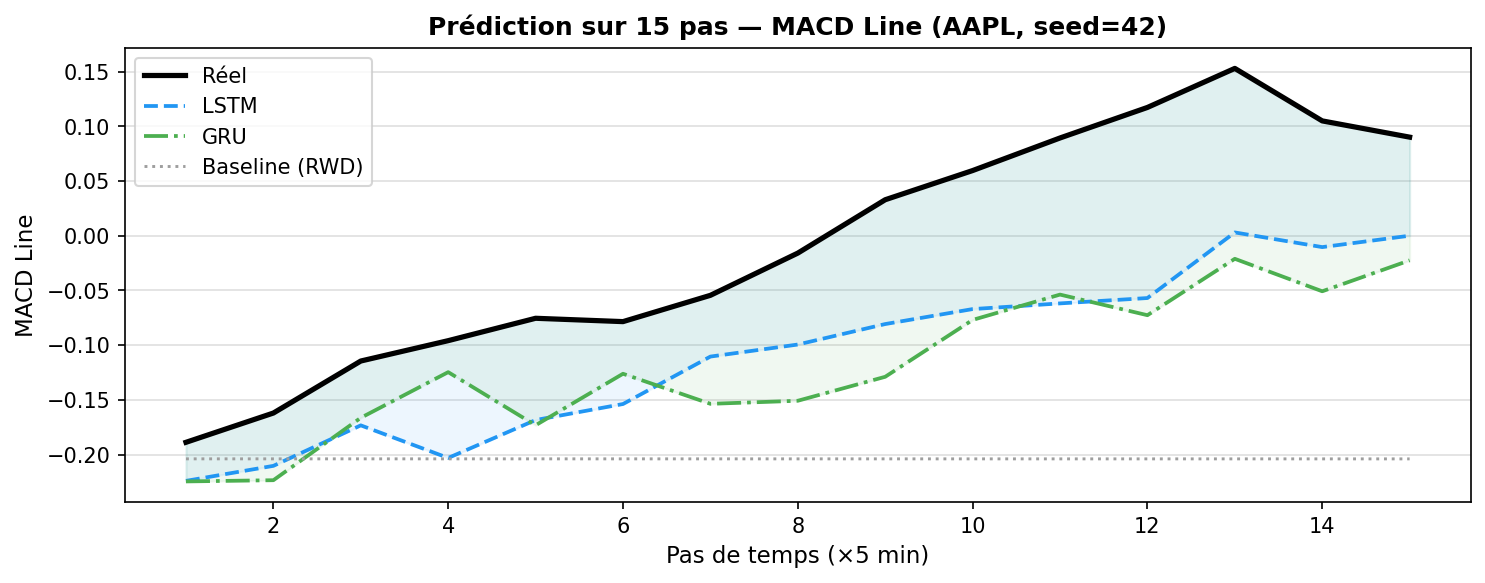
\includegraphics[width=\textwidth]{../figures/fig_pred_macd.png} \\
        \vspace{0.2cm}
        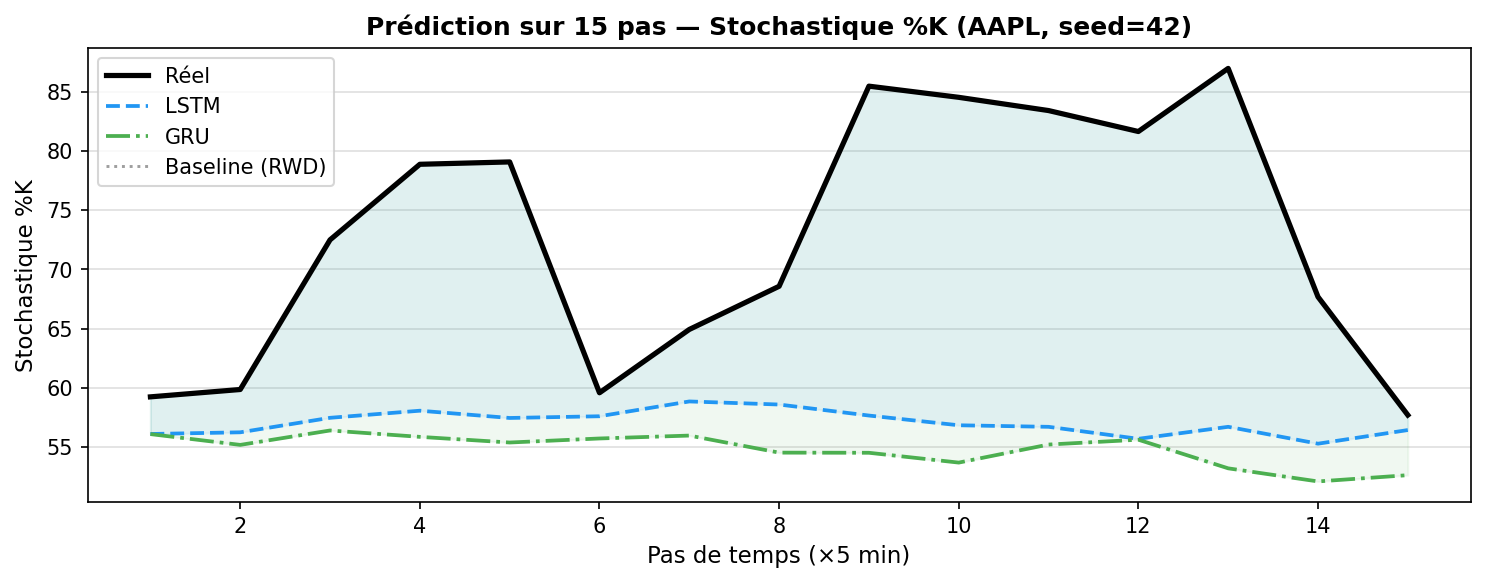
\includegraphics[width=\textwidth]{../figures/fig_pred_stoch.png}
    \end{columns}
\end{frame}

% ---------------------------------------------------------
\begin{frame}{Tester la Robustesse : Cas Journaliers}
    Mais comment le pipeline réagit-il quand on change la brutalité des marchés ?
    
    \vspace{0.3cm}
    \begin{columns}
        \column{0.45\textwidth}
        \textbf{Le Cas MSFT (Retournement)} \\
        Les réseaux basés sur la mémoire sont piégés par la récente chute du cours provoquant l'effondrement intégral des scores du MACD. 
        \vspace{0.2cm}
        \\Pourtant le \textbf{Transformer} survit à l'enfer en devinant la danse millimétrée du Stochastique ($\rho=0.81$ !).

        \column{0.55\textwidth}
        \centering
        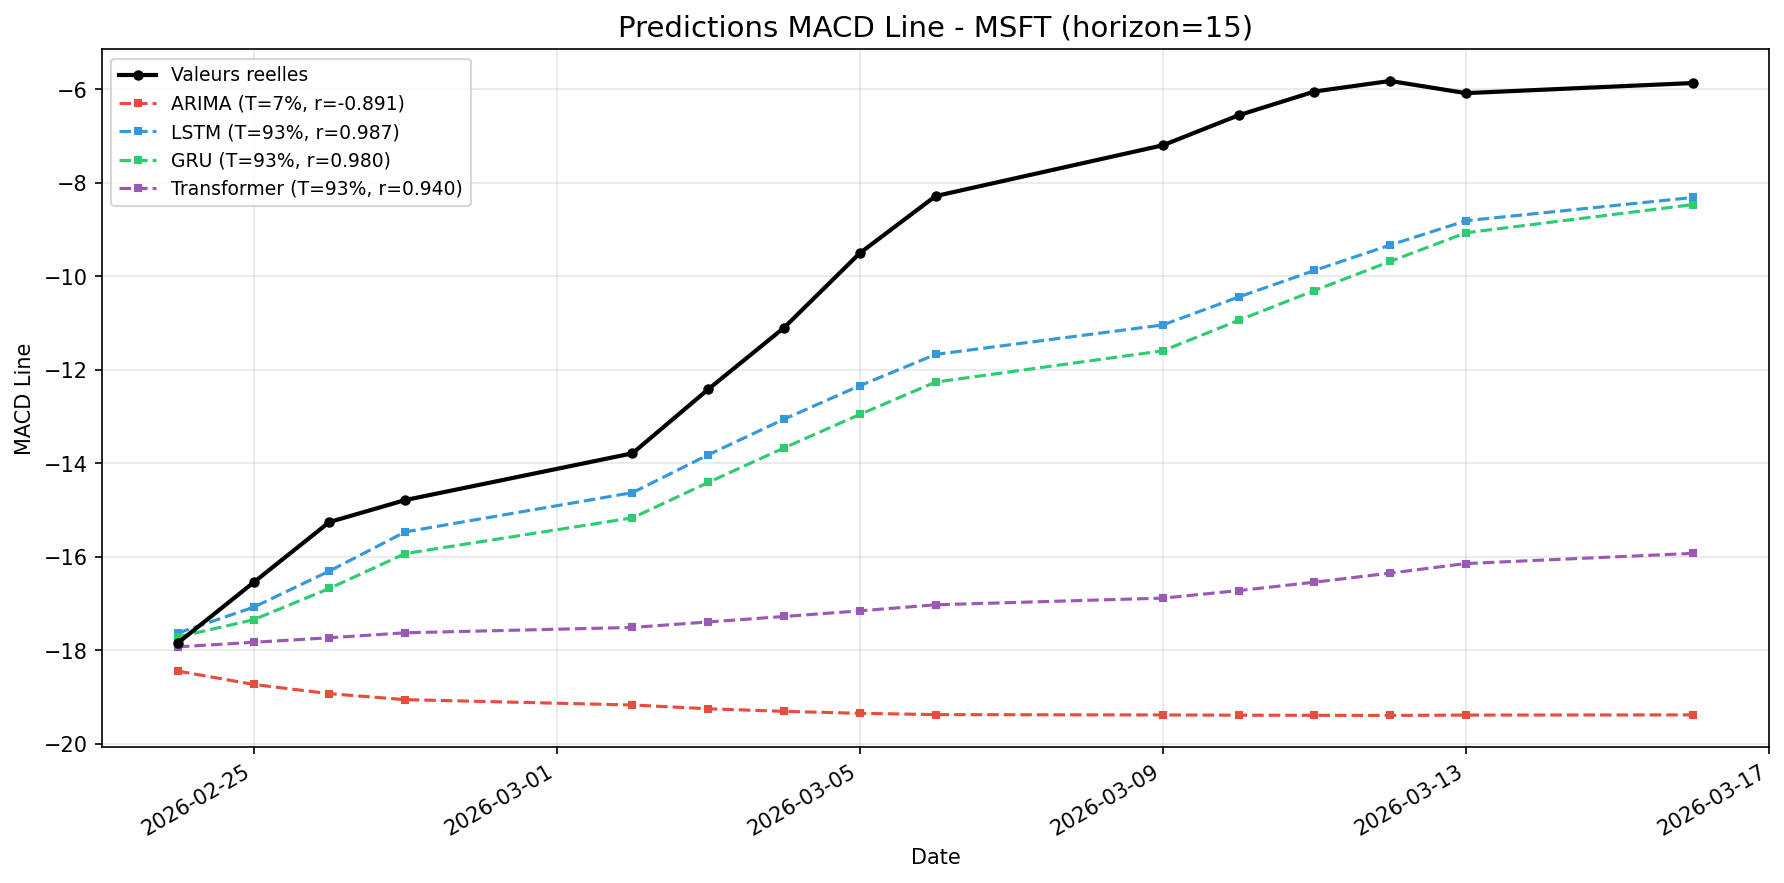
\includegraphics[width=0.9\textwidth]{../figures/MSFT_MACD_Line_predictions.png} \\
        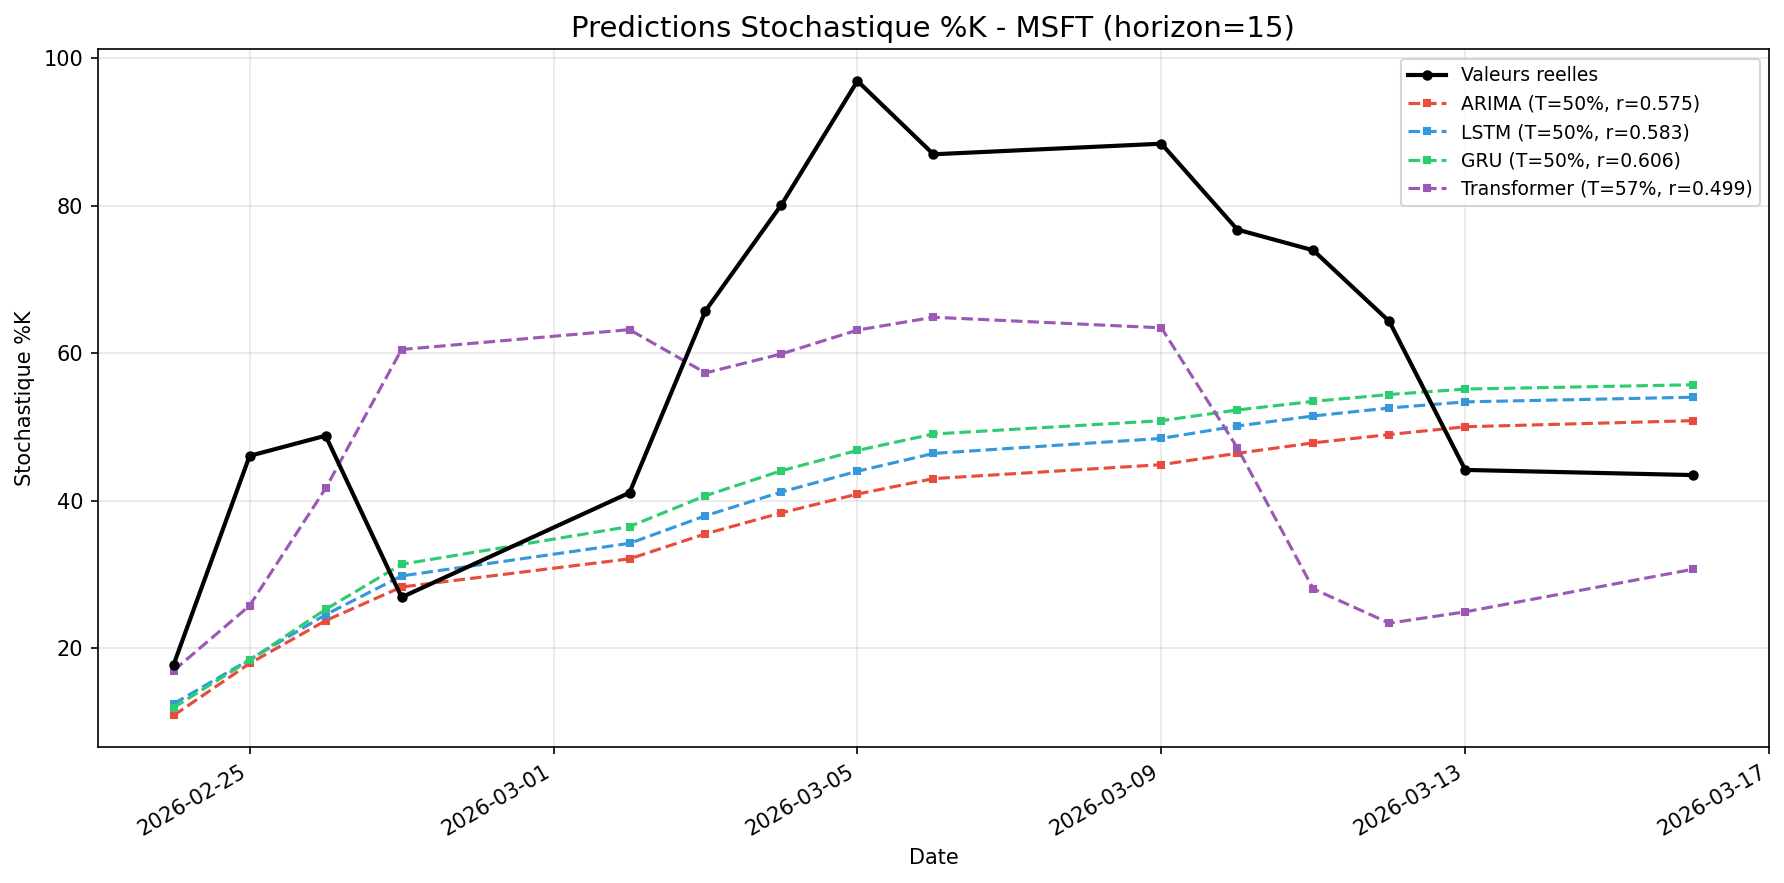
\includegraphics[width=0.9\textwidth]{../figures/MSFT_Stochastique_pctK_predictions.png}
    \end{columns}
\end{frame}

% ---------------------------------------------------------
\begin{frame}{Bilan et Enseignements Multi-Régimes}
    \begin{block}{La Suprématie est un Mythe Contextuel}
        Le choix de la brique de calcul est vital et doit pivoter autour de \textbf{l'actif évalué} :
        \begin{itemize}
            \item \textbf{GRU} $\rightarrow$ Suprématie absolue sur données massives et tendancielles.
            \item \textbf{LSTM} $\rightarrow$ Vital pour enregistrer des dérives sur de puissantes bulles (NVDA).
            \item \textbf{Transformer} $\rightarrow$ Excellent pour le bruit Stochastique, sans doute l'arme ultime une fois accélérée sur des noyaux GPU exclusifs.
        \end{itemize}
    \end{block}

    \vspace{0.3cm}
    \centering
    \alert{\Large Objectif Hackathon pulvérisé avec un max de 0.79 !} \\
    \textit{(Objectif demandé : 0.55)}
\end{frame}

% ---------------------------------------------------------
\begin{frame}[plain]
    \centering
    \vspace{1.5cm}
    {\Huge \textbf{Merci de votre attention !}} \\
    \vspace{0.5cm}
    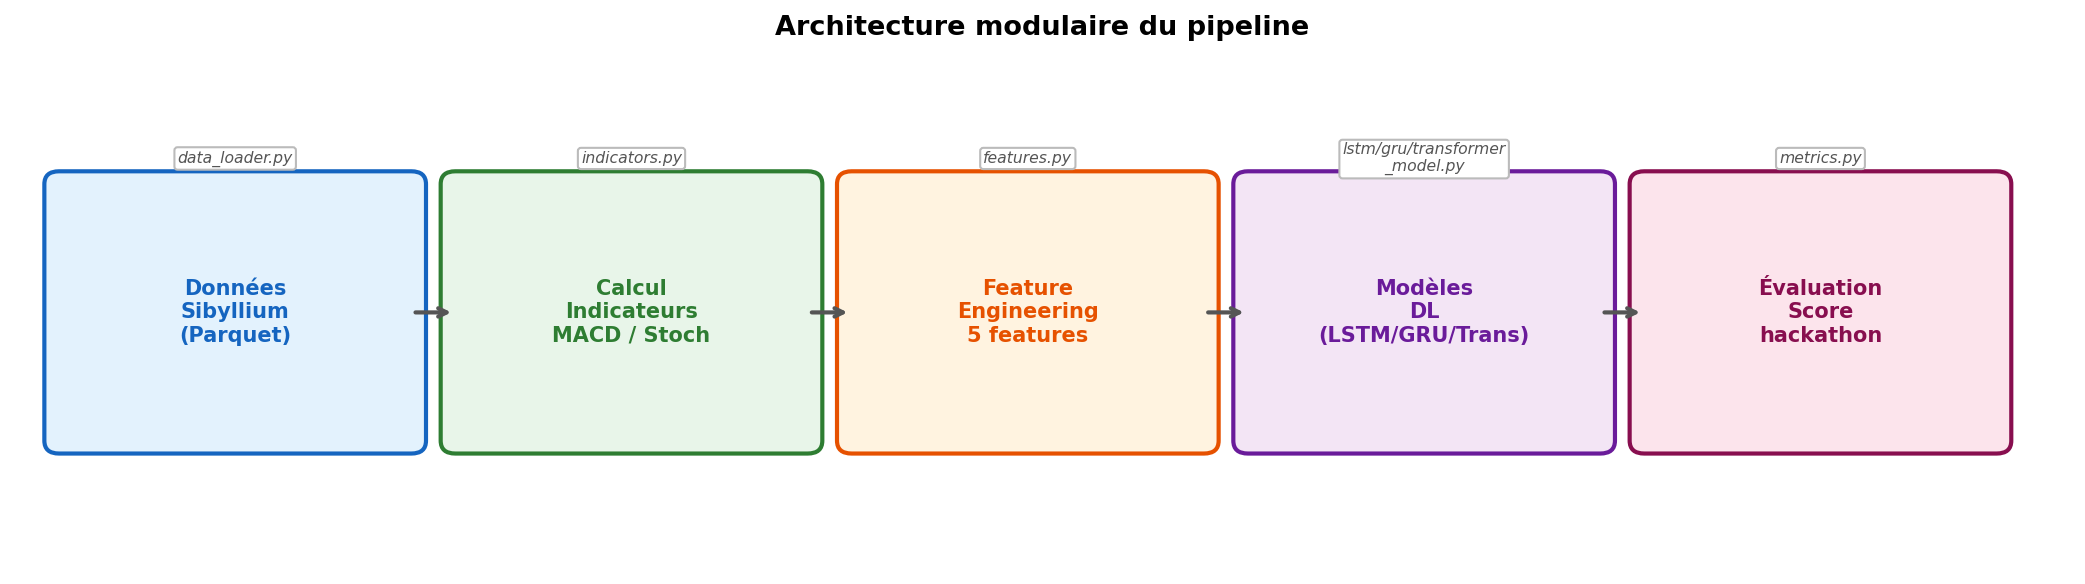
\includegraphics[width=6.5cm]{../figures/fig_pipeline_schema.png} \\
    \vspace{0.5cm}
    \textit{Place à la critique et à vos questions.}
\end{frame}

\end{document}
